\chapter{Design and implementation}

In previous chapter, we introduced Computer Aided Translation, discussing how multiple assistance ways provided within systems implementing this concept  relate to our novel tool that aims to support translators by providing an ability to fix specified parts of the translation using paraphrasing options. Furthermore, we discussed previous paraphrasing approaches highlighting similarities and difference with technique we use to search paraphrases. And finally a brief overview of phrase-based Statistical Machine Translation was provided to introduce origins of the search graph, data structure that we use as main source for paraphrasing.

Current chapter will provide detailed description of work that was carried out during this project. We start by analysing requirements for paraphrasing service within a CAT system. After that an iterational design and implementation process we applied to develop working version of such service. Major design decision that were made during the work on project will be introduced and justified. 

\section{Analysing requirements}

As mentioned earlier, an essential aspect of our paraphrasing approach is that it aims to provide a real-time targeted paraphrase search. Unlike previous efforts discussed by us before, we consider an interactive environment were queries sent by users are executed against our data model and results after being dynamically filtered and ranked using various heuristics are returned to user interface. In this section we list main requirements for our approach that were considered during design stage.

\textbf{Integration with existing CAT software}. Taking into account that most of modern CAT implementations are providing web based service (Caitra, Casmacat, MateCat), we also employed the client-server architecture to design our paraphrasing service. It might be easily attached as a module to the services provided online. Moreover, our service could also be hosted as a standalone service and integrated with desktop translation software by providing an API. This way our paraphrasing assistance might be accessible from all major types of CAT applications.

\textbf{Reusing results of machine translation}. Another important feature of our paraphrasing system is being able to produce paraphrases using only data available as a result of machine translation that provides post-editing assistance, rather requiring any additional paraphrase corpora. We designed our implementation to support translation output generated by Moses []. The process of retrieving and processing search graph will be reviewed by us in [section 3.2].

\textbf{Importance of ranking}. Quality of final ranking of the paraphrasing options is crucial requirement for RePhraser that aims to provide an interactive service. Indeed, basic concepts of Human-Computer Interaction suggest that paraphrasing options displayed to users will be efficient only in case if there count doesn't exceed 7. This means that it's important to rank top results in a way that they will contain at least one good paraphrase. Features that we exploited for ranking as well as a dynamic system of filters and sorters that we applied to improve top results will be described in [section 3.5].  


\textbf{Paraphrasing granularity}. Various levels of paraphrase granularity are studied. In case of entire sentences the task is known \textit{sentential} (or \textit{clausal}) paraphrasing, for shorter items it is called \textit{lexical} (or \textit{phrasal}) paraphrasing. For our project we investigated only lexical paraphrases, motivating this decision by the fact that other assistance tools within a CAT system may already provide multiple translation options for entire sentence, for example results of translation by using different bilingual parallel corpora. We also acknowledge that within scope of lexical paraphrases there is a further separation into two classes that correspond to shorter and longer phrases. Both cases were considered by us during evaluation stage.

We also took into account following study {[]}, which analyses usage patterns of another assistance tool, bilingual concordancer where authors suggest that average length of the input query is 2-3 words. Parallels between this assistance way and ours were discussed in previous chapter and in practice they motivate expectation of average paraphrasing query length to be similar.

\textbf{Realtime experience}. Another requirement for our interactive tool is providing paraphrasing options as fast as possible. Our tool will not be useful at all if it takes it to return results longer that time user spends on manual paraphrasing. Thus we considered time required to generate paraphrases in our evaluation. 

\textbf{Coexistence with manual editing}. While RePhraser aims to be used in order to fix erroneous part in the translation by getting the corrected paraphrase automatically, we acknowledge that final high quality translation cannot be achieved only by using paraphrasing. An ability to manually post-edit translation is crucial and designing our approach we considered that it will be used in an environment where translation could be altered by user at any time.  

\section{Preparing data}

\subsection{Retrieving search graph dump file}

A representation of the search graph, described by us in Section 2.3, could be optionally returned by Moses using \textsf{-output-search-graph FILE} parameter. Resulting text file contains list of hypotheses that were considered during the decoding stage. Each line in the file represent such hypothesis. Contents of file is ordered by sentence identifiers, that appear in the beginning of each line indicating to the sentence that was being translated when the hypothesis formed. The hypotheses are in one of three possible formats.

The \textit{initial hypothesis} refers to the empty hypothesis that is used as starting point in process of hypothesis expansion. This hypotheses have a simple structure and don't carry any additional information:

\begin{verbatim}
0 hyp=0 stack=0
\end{verbatim}

The \textit{regular hypothesis} encodes information about translation decisions that were made by the decoder in a given state. Sample regular hypothesis has following format:

\begin{verbatim}
0 hyp=10 stack=1 back=0 score=-1.497 transition=-1.497 forward=3437
fscore=-8.900 covered=0-0 out=del Parlamento
\end{verbatim}

The line starts with sentence identifier which is followed by a unique hypothesis identifier \textsf{hyp=10}. This identifier is used to reference hypotheses. The stack in which hypothesis is placed identified by \textsf{stack=1}, this is also the number of words covered in original input. The next attribute \textsf{back=0} is a reference to the previous hypothesis, in this case it refers to the initial empty hypothesis. This means that current hypothesis represents the first translation option addition. Overall score of current partial translation is expressed as \textsf{score=-1.497}, which derives from a log-probability which is calculated given machine translation models. The cost of transition to current state is available as \textsf{transition=-1.497}. After finalising the translation, hypothesis attributes are enriched by adding information about the best forward step \textsf{forward=3437} and score \textsf{fscore=-8.900} to the end of the graph. Original sentence coverage information is available in following format \textsf{covered=0-0}, where \textsf{0-0} indicates covered interval.
Finally, the last attribute \textsf{out=del Parlamento} contains the translation option that was added by introducing current hypothesis.

The third type of hypothesis groups \textit{recombined hypotheses}. That are omitted as a result of recombination process that was reviewed by us in Section 2.3.5. Recombined hypotheses have following format

\begin{verbatim}
0 hyp=734 stack=2 back=24 score=-2.684 transition=-1.226 
recombined=731 forward=8037 fscore=-7.962 covered=3-3 out=de Apoyo
\end{verbatim}

Here additional attribute \textsf{recombined=731} indicates to the hypothesis with a better score, with which current hypothesis was recombined.

Another option fetching the information generated during decoding is executing Moses with \textsf{-verbose 3} parameter. This way detailed logs will be provided by the system. The resulting output will contain mostly discarded hypotheses and will not have information about best path that is being added in case of the switch we described earlier. That is why we prefer using the \textsf{-output-search-graph} option instead.

More details are available at [http://goo.gl/6RYbDK]

\subsection{Preprocessing data for paraphrasing}

For initial testing purposes we used Moses to translate set of 3000 Russian sentences from news domain (\textit{newstest2012b}) into English. The resulting search graph dump file was about 5.7GB. In order to process it efficiently we decided to encode information from this file into a relational database. We developed a small Python script that parsed each line in the search graph file and mapped attributes into a dictionary, which was then stored in an SQLite database. The resulting transformation reduced size of our graph representation to 2.3GB. Moreover, main benefit of having our graph stored in a relational database was being able to run SQL queries against it. 

\section{Project design outline}

In this section we want to introduce high-level structure of the project listing it's main components and their short descriptions. Following sections will provide more details about implementation of these components. As it was mentioned before, our service designed using client-server architecture. While client-side implementation may vary depending on particular CAT software within which paraphrasing service is provided, and integrating our solution with a particular CAT system was out of the scope of current work, we have implemented simple web based mock interfaces to test usability and feasibility of our tool. 

Our server-side implementation is also designed as a proof of the concept and currently supports only paraphrasing of sentences that are available in the preprocessed search graph database. The production of this database graph was reviewed in previous section and it could be executed as an initialisation step triggered after the machine translation for post-editing is produced. Simple sequence of components that are used to process paraphrasing requests are illustrated in Figure 3.1.

\begin{figure}
 \centering 
 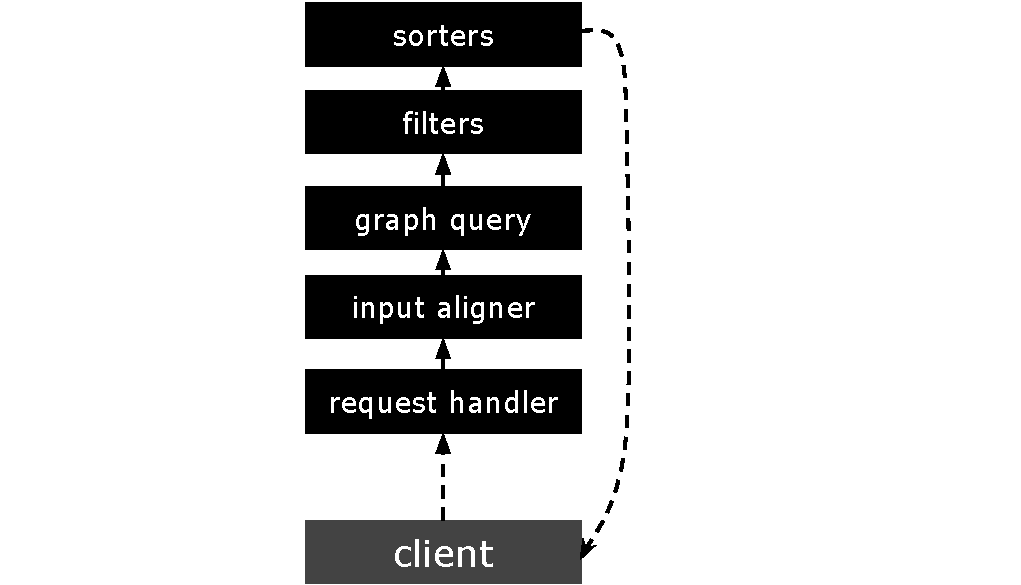
\includegraphics{g/system-outline.pdf}
 \caption{Paraphrasing request handling}
\end{figure}

\subsection{Sending requests from client}

Simple integration of paraphrasing service into a Computer Aided Translation interface will require adding a button labeled ``Paraphrase Selection'' near the active translation edition box. The button will be enabled only in case if user selects part of translation text using mouse cursor. Once clicked, button will fire an event that will send a paraphrasing request. The requests from clients are sent over HTTP protocol using AJAX technology. Figure 3.2 illustrates English to Russian translation setup in CASMACAT system, user selects part of translation provided for post-editing and paraphrase button is activated.

\begin{figure}
 \centering
 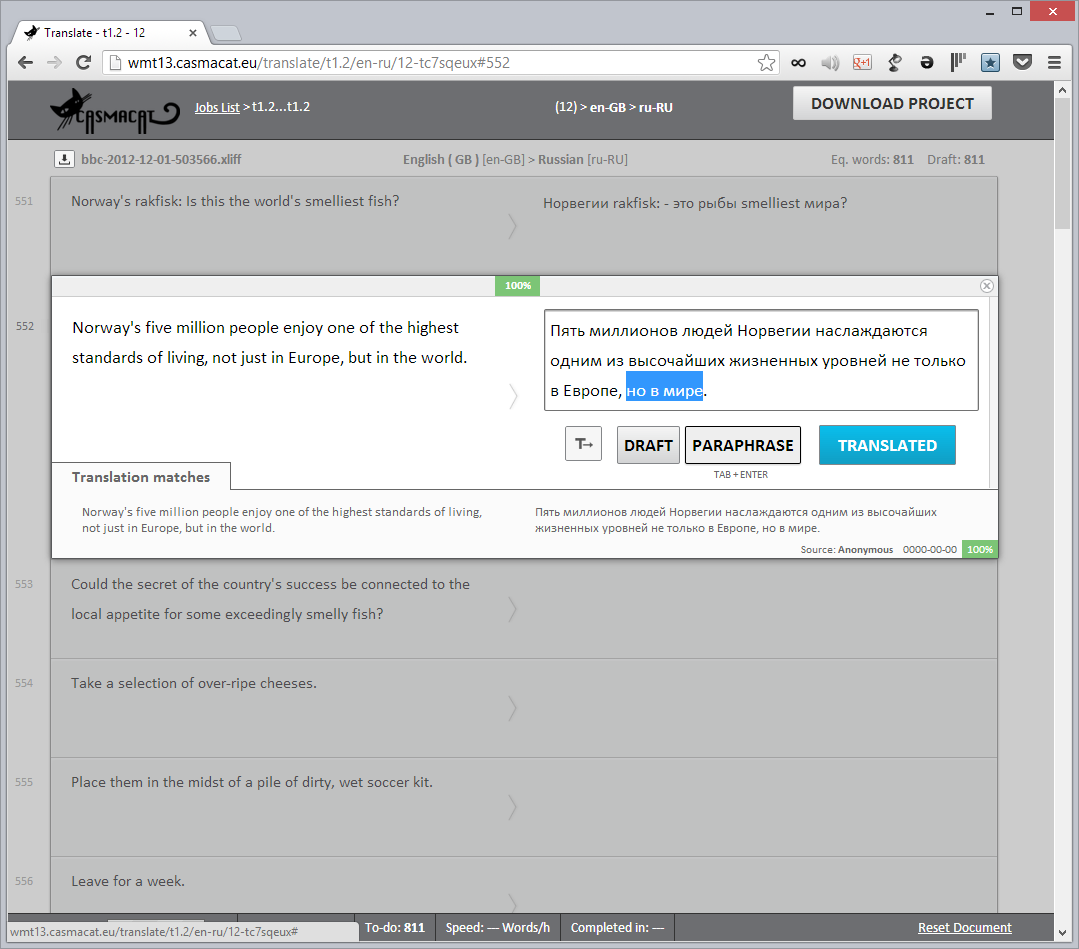
\includegraphics[scale=0.5]{g/screenshot.png}
 \caption{Sample screenshot of paraphrasing client UI}
\end{figure}

\subsection{Request handler}

The role of request handler is simply to intercept messages from client-side and to transform them into native easy to use data structures. In our implementation we used Werkzeug WSGI toolkit which is freely available for Python.

\subsection{Input aligner}

Before user's paraphrasing query is executed against our graph database, it is being aligned with corresponding part original sentence in source language. Main reasoning behind this step is making sure that our paraphrasing will not produce duplicated translation by capturing partial translation of a phrase that was not originally requested by user. In this process we are interested only in retrieving pointers to original sentence parts that correspond to user's selection, fetching original language phrases is not required.

\subsection{Graph query execution}

Having required information about coverage, system executes a query against search graph database. This is achieved by transforming search constraints into an SQL query. Depending on phrase length and other phrase specific features several sequential SQL queries could be executed. Results represent a list of unfiltered translation options that are have high probability of being suitable paraphrases to user's selection. Each translation option is paired with data about corresponding hypothesis scores, that are used in further stages of paraphrasing workflow.

\subsection{Filters and sorters}

Results retrieved from database are usually very redundant and have formatting issues. Thus the next step filtering them and after that using scoring function to generate final ranking. This step encapsulates the most significant part of paraphrasing algorithm. In order to experiment with various filtering and ranking techniques we have implemented a dynamic system of attachable filters and sorters. This way we were able to easily produce multiple variations of our approach and evaluate all of them against one test suite. Importantly, another benefit of this dynamic modular system is that depending on user's query we can execute different sets of filters and sorters. For example, as we will see some filters could be efficiently used only for short phrases, while others are suitable for long inputs. 

\section{Implementation details}

\bibliography{library}
